\documentclass{article}
\usepackage{mhchem}
\usepackage{amsmath}
\usepackage{enumitem}
\usepackage{graphicx}
\usepackage{adjustbox}
\graphicspath{{graphics/}}
\begin{document}

\author{Elston Almeida}
\title{Chemistry Grade 12 \\ Chapter 7 Review}
\maketitle

\setcounter{section}{7}

\subsection{Chemical Equilibrium}

\begin{paragraph}
  \noindent
  The state where the rate of forward reaction is equal to o the rate of reverse reaction is called chemical equilibrium. The left right arrows denote a reaction at equilibrium (\ce{<=>}). Equilibrium can only truely occur in a closed system or the reverse reation cannot take place.
\\

When at equilibrium, all macroscopic quailities such as color, conductivity, pH, density, etc. Remain the same. However the solution may seem static, it is rather dynamic. On the molecular level the molecules are constantly reacting in a forwards and reverse reaction $eq^m$
\\

This does not mean that the concentrations of the reactants and products are equal, instead it means that their concentrations stay constant, As that would mean the reaction is in the dynamic state of constantly producing and consuming the same amount (rate of forward and reverse reactions are equal). On a graph, the concentrations of the products and reactants have to be a straight line. $m=0, d(M(x))/dx=0$
\\
\vspace{2pc}

\begin{adjustbox}{center}
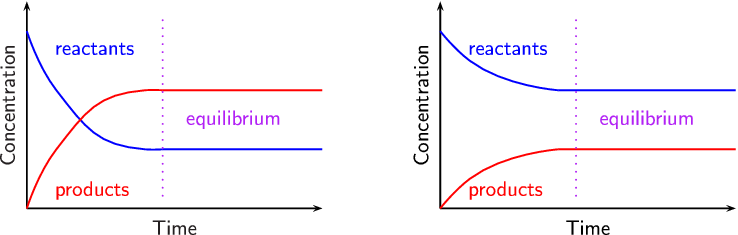
\includegraphics[scale=0.5]{eqGraph.png}
\end{adjustbox}

\newpage
\subsection{Equilibrium Law and the Equilibrium Constant}

\begin{center}
\ce{ A + B <=> C + D}
\end{center}

\begin{equation}
  K_c = \frac{[A][B]}{[C][D]}
\end{equation}
\\

\noindent
$K_c$ is the equilibrium constant and is the simple ratio of products to reactants.
\\

$K_c$ must only be taken at the equilibrium. It is seen as the constant for the forward reaction, similarly, the reciprocal of it is the value of the reverse reaction.

\begin{equation}
  K_{cf} = \frac{1}{K_{cr}} \hspace{4pc} K_{cr} = \frac{1}{K_{cf}}
\end{equation}

$K_{c f}$ and $K_{c r}$ defines the forward and reverse reactions respectivly. $K_c$ does not include solids or liquids, only aqueous solutions and gasses. This is because solids and liquids have a fixed density and therfore are ommited from the expression.
\\

\noindent
The very important idea to note is the equilibrium constant is only dependent on the temperature.

\setcounter{subsection}{3}

\subsection{Qualitative Changes to Equilibrium}

*If the rates of temperature, pressure, or concentration change under equilibrium conditions, this would change the rates of the forward and reverse reactions.
\\

In Accordance to \textbf{Le Chatellier's Principal}, if one of these conditions change the chemical will undergo an equilibrium shift, chemical intertia. It will resist the change and start trying to reverse the effect. Think of it as a see saw trying to constantly be perfectly level. If the concentration increases the reaction shifts to the side to consume more reactant, and vise versa.\\

When pressure is increased the reaction will favour the side where there are less amount of reactants, and vise versa. This can also be a factor when volume is changed due to Boyle's law, as pressure is inversely related to volume.\\

When temperature is increased, the reaction will favour the side to consume all the added thermal energy and the opposite effect will occur if the opposite was to occur. Only if temperature is a product or reactant in the reaction.\\

 However, note that the $K_c$ does not change for pressure, or concentration, only temperature. Thus why $K_c$ values are always reported with the temperature. $*$ There is no effect on the system when introduced to an inert gas or a catalyst (It is to be noted that when a catalyst is added the rate of forward and reverse reactions occur equally faster).\\


\subsection{Quantitative Changes to Equilibrium}

The ratio of the product over the reactants at any time other than equilibrium is considered as the Q value. The Q value helps determine the type of shift required for the system to reach equilibrium.

\begin{align*}
  Q &= K & & \text{system is at Equilibrium}    \\
  Q &> K &&  \text{system needs to shift left}  \\
  Q &< K &&  \text{system needs to shift right}
\end{align*}

\subsection{Solubility Equilibria and the $K_{sp}$ Value}

\noindent
3 Different types of Equilibra:

\begin{description}
\item[$\bullet$] Phase Equilibrium: The differnce physical states of a pure substance in an enclosed system.
\item[$\bullet$] Chemical Reaction Equilibrium: Between reactants and products of a chemical reaction in a closed reaction.
\item[$\bullet$] Solubility Equilibrium: Between a solvent and a solute in a saturated closed system.
\end{description}
%% \\
At $eq^m$ water molecules and ions still collide with the surface of the crystal, but the \textbf{rate of dissolution equals the rate of crystalization}.

\begin{center}

\ce{AB(s) <=> A^+(aq) + B^-(aq) }

\end{center}

Solubility product constant $K_{sp}$ can help determine how soluble is an item. Measured by saturating solutions of item or percipitate it out of solution. Generally, ionic compounds have a low $K_{sp}$ value, and compounds with high solubility do not percipitate and do not form equilibria.
\\

In this we can use the Q value (now called \textbf{Trial Ion Product}) to determine if a product will percipitate, you take the ions forming the percipitate and find the Q of the ion(s) specific reaction, then compare the Q with the value of $K_{sp}$.

\begin{align*}
  Q &= K_{sp} && \text{Percipitate will not form, saturated solution}   \\
  Q &> K_{sp} &&  \text{Percipitate will form, supersaturated solution}  \\
  Q &< K_{sp} &&  \text{Percipitate will not form, undersaturated solution}
\end{align*}

The common ion effect is to reduce the solubility of an ionic compound by adding a common ion, this can be described by Le Chatellier's Principal as the reaction tries to balance itself.\\

\scriptsize{I fell asleep making this and I did not have any auto correct, sorry for any spelling mistakes}

\end{paragraph}

\end{document}
